\documentclass{article}
\usepackage[T1]{fontenc}
\usepackage{lmodern}
\usepackage{graphicx}
\usepackage{amsmath,amssymb}
\usepackage[a4paper,margin=2cm]{geometry}
\usepackage[absolute,overlay]{textpos}
\setlength{\TPHorizModule}{1mm}
\setlength{\TPVertModule}{1mm}
\usepackage[indonesian]{babel}
\usepackage{hyperref}
\setlength{\emergencystretch}{2em}
% unit: Halaman 6

\begin{document}

% === Halaman 6 (llm) ===

\vspace{192.46mm}

Joan Daemen and Vincent Rijmen, the designers of the Advanced Encryption Standard
(Sumber: \url{https://medium.com/@stkgroup/what-is-the-advanced-encryption-standard-and-how-does-it-work-abd1ec582df8})

% deskripsi: Foto Joan Daemen dan Vincent Rijmen, perancang Advanced Encryption Standard (AES).
% bbox normalisasi: [0.1970, 0.0540, 0.7650, 0.7020]
\begin{textblock*}{119.28mm}(41.37mm,16.04mm)
\noindent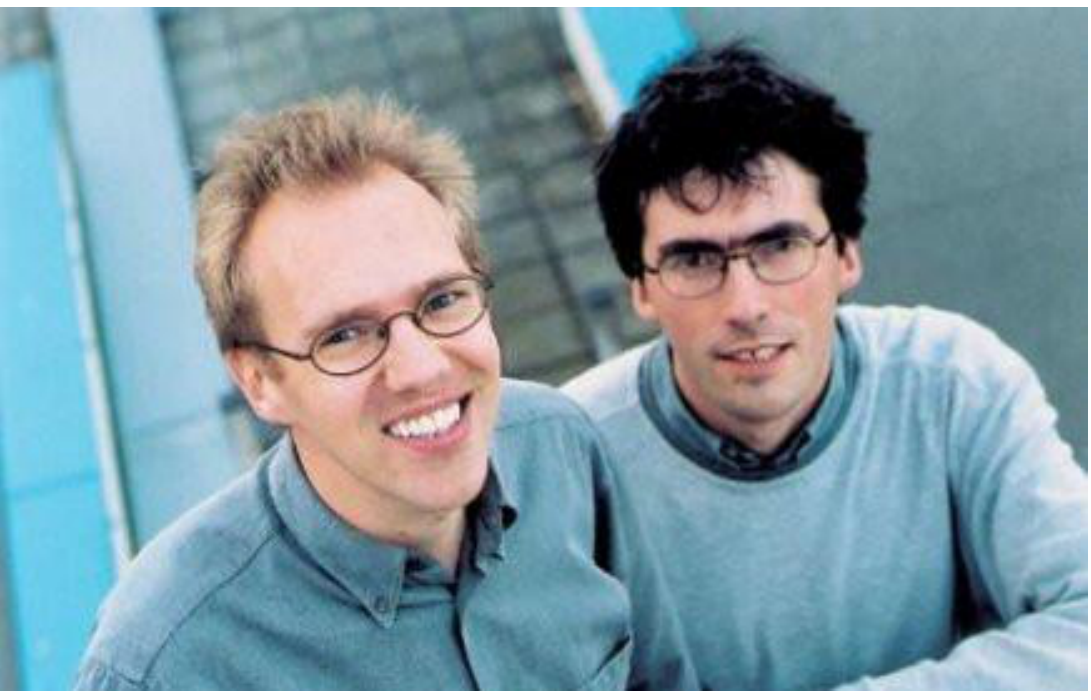
\includegraphics[width=119.28mm,height=192.46mm]{../../images/llm/page_006_img_01.png}%
\end{textblock*}

\end{document}
